\documentclass{article}
\usepackage{geometry}
\usepackage[T1]{fontenc}
\usepackage[utf8]{inputenc}
\usepackage[pdftex]{graphicx}
\usepackage{multicol}
\usepackage{url}
\usepackage{algorithmic}
\usepackage{algorithm}
\usepackage{amsmath}
\usepackage{setspace}

\onehalfspacing

\geometry{a4paper}

\title{Hybrid Rasterization / Ray Casting for Volumetric Lighting}
\author{Richard Monette}

\begin{document}
\maketitle
\pagebreak[4]
\tableofcontents
\pagebreak[4]

\section{Introduction}

One of the most compelling aspects of computer graphics is the rendering of so called participating media phenomena such as smoke, fog and clouds. Esthetically pleasing treatment of these phenomena is critical to achieving high quality computer graphics imagery. This thesis presents a high quality, computationally efficient technique for rendering such participating media. Specifically, we introduce a new method for computing volumetric lighting solutions for participating media which is modeled by particle data sets, as opposed to traditional grid based representations. We seek to render particle based participating media because a range of modern fluid dynamics computation solutions use particle based data sets, instead of traditional grid based density tracking. Our technique is capable of computing volumetric lighting for particle data sets consisting of millions of particle for an arbitrary number of lights of various types and exhibits linear algorithmic complexity. 

In Chapter 2, we begin by establishing a theoretical basis which describes the various types of interactions which light may have with participating media. A survey of the relevant research is provided in Chapter 3. We then present a detailed definition of the problem which our technique addresses, followed by the implementation details, results and conclusion.

\section{Theoretical Overview}

In general, computer graphics solutions make the assumption that the scenes to be rendered are made up of a collection of solid surfaces existing in a vacuum. This assumption greatly simplifies rendering since, in a vacuum, radiance (the measure of brightness and color of a single ray of light\cite{RTR3}) is constant along any path between the surfaces, lights and virtual cameras. However, this assumption, while beneficial in terms of reducing computational complexity, has the shortcoming of preventing the rendering of effects such as attenuation and scattering of light due to participating media, such as fog and smoke or atmospheric effects.

To capture such effects, we must use those techniques which calculate the interaction of the light with the participating media present in the scene. Participating media is that matter, such as water droplets (in the case of fog) or dust part particles (in the case of smoke), which will affect the behavior of light by changing the direction in which it travels and the amount of energy it carries due to processes such as scattering and absorption.

Participating media is characterized as being either homogeneous or in-homogeneous in nature. A homogeneous media is uniform throughout the scene whereas an in-homogeneous media spatially varies in properties such as density, color or other attributes.

\subsection{Participating Media Interaction Processes}

Four main processes affect the distribution of radiance in a scene in the presence of some participating media:

\begin{itemize}

\item Absorption - reduction in radiance due to the conversion of light to another form of energy such as heat
\item Emission - radiance that is added to the environment from luminous particles
\item In-Scattering - radiance that interacts with particles, changing direction such that it then travels along the viewing ray to the camera
\item Out-Scattering - radiance that interacts with particles, changing direction such that it does not travel along the viewing ray to the camera

\end{itemize}

Next, we examine each of these processes in detail.

\subsubsection{Absorption}

Absorption is the process by which radiance interacts with participating media reducing the total transmitted radiance. Absorption is measured using the absorption coefficient $\sigma_{a}$ which is the probability density that light is absorbed per unit distance traveled in the medium. In the case on an in-homogeneous medium this absorption coefficient may be spatially varying, whereas it will be uniform in a homogeneous medium. Typically, this value also varies with respect to the frequency of the light (i.e. higher wavelengths interact more with the participating media resulting in a quicker absorption).

\begin{figure}[h!]
	\centering
	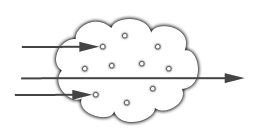
\includegraphics[scale=0.75]{Images/Absorption}
	\caption{Incident radiance is reduced due to absorption resulting in less outgoing radiance.}
\end{figure}

Given some incident radiance $L_{i}(p,\omega)$, at position $p$ traveling along vector $\omega$, we find the change in outgoing radiance $L_{o}(p,\omega)$ after the absorption interaction with the participating media using the following equation:

\begin{equation}
dL_{o}(p,\omega) = -\sigma_{a}(p,\omega)L_{i}(p,-\omega) dt
\end{equation}

\subsubsection{Emission}

Emission increases the amount of radiance traveling along some path through a participating media due to the conversion of energy into visible light by chemical, thermal or other means. For example, consider the glowing hot gas of a torch. The burning gas releases energy, some of which will be in the form of visible light.

\begin{figure}[h!]
	\centering
	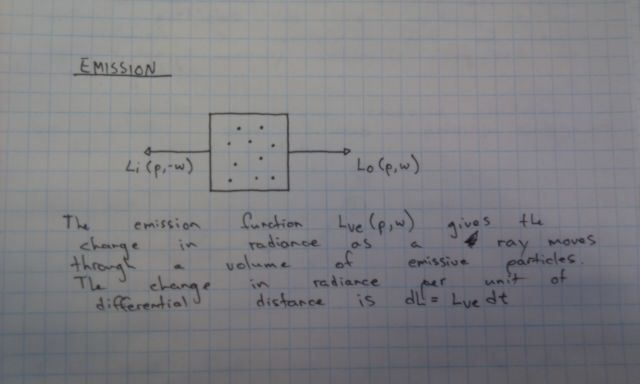
\includegraphics[scale=0.5]{Images/Emission}
	%\caption{Solving Single Scattering with Ray Tracing}
\end{figure}

\subsubsection{Out-Scattering}

As a beam of light passes through some participating media, it may intersect with the particles that constitute that media. This interaction can cause the light to change the direction in which it is traveling. The effects of this scattering are two fold. The first outcome is that the total radiance will be reduced to the out-scattering of light energy. However, it is also possible that light will enter the medium and be scattered such that it is added to that which reaches the virtual camera. This outcome, where light is added, is referred to as in-scattering.
\newline \newline
The probability of an out-scattering event occurring per unit distance is given by the scattering coefficient, $\sigma_{s}$. As with the absorption coefficient, the reduction in radiance along a differential length of $dt$ due to out-scattering is given by:
\newline \newline
\begin{equation}
dL_{o}(p,\omega) = -\sigma_{s}(p,\omega)L_{i}(p,-\omega) dt
\end{equation}
\newline
Thus, the total reduction in radiance due to absorption and out-scattering is the sum of $\sigma_{a} + \sigma_{s}$. This combined effect of absorption and out-scattering is called attenuation or extinction. For convenience, the sum of these two coefficients is denoted by the attenuation coefficient $\sigma_{t}$:
\newline \newline
\begin{equation}
\sigma_{t}(p,\omega) = \sigma_{a}(p,\omega) + \sigma_{p,\omega}(p,\omega)
\end{equation} 
\newline
Given the attenuation coefficient $\sigma_{t}$, the differential equation describing overall attenuation,
\newline \newline
\begin{equation}
\frac{dL_{o}(p,\omega)}{dt} = -\sigma_{t}(p,\omega)L_{i}(p,-\sigma),
\end{equation}
\newline
can be solved to find the beam transmittance, which gives the fraction of radiance that is transmitted between two points on a ray:
\newline \newline
\begin{equation}
T_{r}(p\rightarrow p') = e^{-\int_d^0 \sigma_{t}(p+t\omega,\omega)dt}
\end{equation}
\newline
where $d$ is the distance between $p$ and $p'$, $\sigma$ is the normalized direction vector between them and $T_{r}$ denotes the beam transmittance between $p$ and $p'$. Note that the transmittance is always between zero and one. Thus, if exitant radiance from a point $p$ on a surface in a given direction $\sigma$ is given by $L_{0}(p,\sigma)$, after accounting for extinction, the incident radiance at another point $p'$ in direction $-\sigma$ is
\newline \newline
\begin{equation}
T_{r}(p\rightarrow p')L_{o}(p,\sigma)
\end{equation}
\newline
Two useful properties of beam transmittance are that transmittance from a point to itself is one ($T_{r}(p\rightarrow p) = 1$ and in a vacuum $T_{r}(p\rightarrow p') = 1$ for all $p'$. Another important property, which is true in all media, is that transmittance is multiplicative along points on a ray:
\newline \newline
\begin{equation}
T_{r}(p\rightarrow p'') = T_{r}(p\rightarrow p')T_{r}(p'\rightarrow p''),
\end{equation}
\newline
for all points $p'$ between $p$ and $p''$. This property is important for volume scattering implementations, since it makes it possible to incrementally compute transmittance at many points along a ray by computing the product of each previously computed transmittance with the transmittance for its next segment.
\newline \newline
The negated exponent in $T_{r}$ is called the optical thickness between two points. It is denoted by the symbol $\tau$:
\newline \newline
\begin{equation}
\tau(p\rightarrow p') = \int_0^d\sigma_{t}(p+t\omega, -\omega)dt
\end{equation}
\newline
In a homogeneous medium, where $\sigma_{t}$ is constant, $\tau$ is trivially evaluation and yields Beer's law:
\newline \newline
\begin{equation}
T_{r}(p \rightarrow p') = e^{-\sigma_{t}d}
\end{equation}

\begin{figure}[h!]
	\centering
	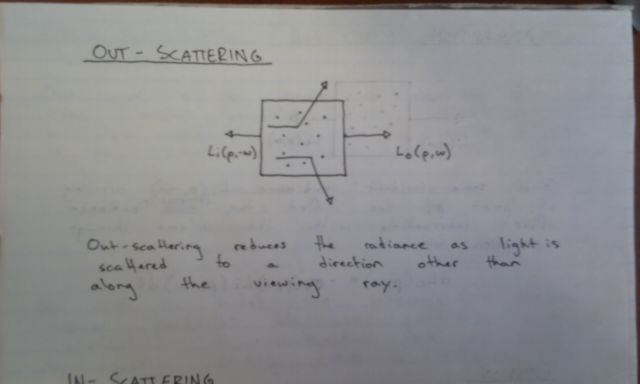
\includegraphics[scale=0.5]{Images/OutScattering}
	%\caption{Solving Single Scattering with Ray Tracing}
\end{figure}

\subsubsection{In-Scattering}

While out-scattering reduces radiance along a ray due to radiance scattering out in different directions, in-scattering accounts for increased radiance due to radiance scattering in from other directions.

The total radiance added per unit distance due to in-scattering is given by the source term $S$:

\begin{equation}
dL_{o} = S(p,\omega)dt
\end{equation}

which accounts for the increase in radiance from both emission and in-scattering:

\begin{equation}
S(p,\omega) = L_{ve}(p,\omega) + \sigma_{s}(p,\omega)\int_{S^{2}}p(p,-\omega'\rightarrow\omega)L_{i}(p,\omega')d\omega'
\end{equation}

This equation states that the total added radiance is the emitted radiance plus all the direct lighting radiance $L_{i}$ that is being in-scattered from all directions.

\begin{figure}[h!]
	\centering
	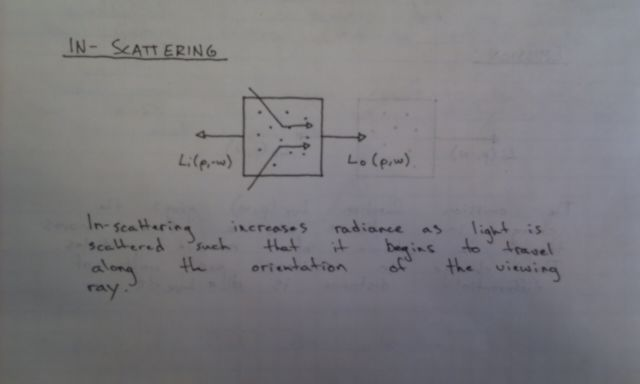
\includegraphics[scale=0.5]{Images/InScattering}
	%\caption{Solving Single Scattering with Ray Tracing}
\end{figure}

\subsection{The Equation of Transfer}

The equation of transfer is the fundamental equation that governs the behavior of light in a medium that absorbs, emits and scatters radiation.\cite{Chandrasekhar60} It accounts for all of the volume scattering processes, which are; absorption, emission and in- and out-scattering. These factors provide an equation that describes the distribution of radiance in an environment. In fact, the light transport equation is a specialized case of the equation of transfer, which has been simplified by the removal of consideration of participating media and specialized only to scattering from solid surfaces.\cite{Arvo93transferequations}

The equation of transfer is an integro-differential equation that describes how the radiance along a beam changes at a point in space. It can be transformed into a pure integral equation that describes the effect of participating media from the infinite number of points along a line. It can be derived in a straightforward manner by subtracting the effects of the scattering processes that reduce energy along a beam (absorption and out-scattering) from the processes that increase energy along it (emission and in-scattering). 

We recall that the source term gives the change in radiance at a point $p$ in a particular direction $w$ due to emission and in-scattered light from other points in the medium:

\begin{equation}
S(p,\omega) = L_{ve}(p,\omega) + \sigma_{t}(p,\omega)L_{i}(p,-\omega)dt
\end{equation}

The source term accounts for all of the processes by which radiance is added to a ray.

The attenuation coefficient, $\sigma_{t}(p,\omega)$, accounts for all processes that reduce radiance at a point: absorption and out-scattering. The differential equation that describes this effect is

\begin{equation}
dL_{o}(p,\omega) = -\sigma_{t}(p,\omega)L_{i}(p,-\omega)dt
\end{equation}

The overall differential change in radiance at a point $p'$ along a ray is found by adding these two effects together to get the integro-differential form of the equation of transfer (the equation is integro-differential due to the integral over the sphere in the source term):

\begin{equation}
\frac{\theta}{\theta t}L_{o}(p,\sigma) = -\sigma_{t}(p,\sigma)L_{i}(p,-\sigma) + S(p,\sigma)
\end{equation}

With suitable boundary conditions, this equation can be transformed into a purely integral equation. For example, if one was to assume that there are no surfaces in the scene such that the rays are never blocked and have an infinite length, then the integral equation of transfer would be

\begin{equation}
L_{i}(p,\omega) = \int_0^\infty T_{r}(p' \rightarrow p)S(p', -\omega)dt
\end{equation}

where $p' = p + \omega$. The meaning of this equation is reasonably intuitive: it states that the radiance arriving at a point from a given direction is contributed to by the added radiance along all points along the ray from the point. The amount of added radiance at each point along the ray that reaches the ray's origin is reduced by the total beam transmittance from the ray's origin to the point.

In a more likely scenario, where there are reflecting and/or emitting surfaces in the scene, rays won't necessarily have infinite length and the surface that a ray hits affects its radiance, adding outgoing radiance from the surface at the point and preventing radiance from points along the ray beyond the intersection from contributing to radiance at the ray's origin. If a ray $(p,\omega)$ intersects a surface at some point $p_{0}$ a distance $t$ along the ray, then the integral equation of transfer is

\begin{equation}
L_{i}(p,\omega) = T_{r}(p_{0} \rightarrow p)L_{o}(p_{0}, -\omega) + \int_0^t T_{r}(p' \rightarrow p)S(p', -\omega)dt'
\end{equation}

where $p_{0} = p + t\omega$ is the point on the surface and $p' = p + t'\omega$ are points along the ray.

This equation describes the two effects that contribute to radiance along the ray. First, reflected radiance back along the ray from the surface is given by the term $L_{o}$, which gives the emitted radiance and reflected radiance from the surface. This radiance may be attenuated by the participating media; the beam transmittance from the ray origin to the point $p_{0}$ accounts for this. The second term accounts for the added radiance along the ray due to volume scattering and emission, but only up to the point where the ray intersects the surface; points beyond that one don't affect the radiance along the ray.

\subsection{Volume Representation}

In order to render participating media, its properties must be tracked throughout the spatial extent of the volume in which it resides. 

\subsubsection{Eulerian / Grid Based}

Traditionally fluid simulations have been conducted using a grid to track density.
\newline \newline
A major disadvantage of using a uniform grid for simulation is that memory is required even for those cells in the grid which are empty. As a result, significant amounts of memory may be required in order to get a simulation which captures sufficient detail and spatial extents.
\newline \newline
In the case of rendering volumes which are represented by grids it is possible to sample the density for a given cell simply by accessing the memory representing this location. This is a major advantage as this access is typically O(1) (constant time).

\subsubsection{Lagrangian / Particle Based}

An alternative method for tracking the properties of some participating media throughout the spatial extent of the volume in which it resides is to consider that participating media to be composed of a number of discrete particles. Typically each particle will be characterized by its position and velocity.

Particle based methods have the advantage of not needing to use computer memory in order to store information about where there is no density. For example, consider a large room through which a cloud of smoke is traveling. Using a uniform grid, it would be necessary to have memory tracking that there is no smoke present in the vast majority of the spatial extent. Given that computer memory is not unlimited, it is very possible that it would not be possible to use a fine enough grid to resolve the fine details of the smoke without surpassing available memory. In contrast, a particle based system would only need to store the information about the location of the particles that are actually representing the smoke.

\subsection{Ray Marching}

Except for cases where participating media is homogeneous and has a uniform isotropic scattering function, the volume rendering function is solved using numerical integration. This integration can be performed using a technique called ray marching\cite{Levoy:1990:ERT:78964.78965} which takes steps through the participating media and evaluates each segment. Each segment has a length of $\Delta x$ and it is assumed that for this length the incoming light and properties of the participating media are constant. Based upon these assumptions, the radiance for a given segment due to direct illumination can be calculated as:

\begin{equation}
L(x, w) = \displaystyle\sum_{l}^{N}L_{l}(x,w_{l}')p(x,w_{l}',w)\sigma_{s}(x)\Delta x + e^{-\sigma_{t}\Delta x}L(x + w\Delta x,w)
\end{equation}

where $N$ is the number of lights in the scene and $L_{l}$ is the radiance from each light source. The first term sums the radiance contribution from a segment and second term accounts for that radiance which is coming from the previous segments. For a participating media volume of finite size, ray marching can be used to compute the total radiance from direct illumination by recursively calling the above formula:

\begin{equation}
L_{n+1}(x, w) = \displaystyle\sum_{l}^{N}L_{l}(x,w_{l}')p(x,w_{l}',w)\sigma_{s}(x)\Delta x + e^{-\sigma_{t}\Delta x}L_{n}(x + w\Delta x,w)
\end{equation}

\subsection{Classic Volume Rendering Techniques}

\subsubsection{Ray Tracing Methods}

The classic method for rendering with participating media is to extend the traditional ray tracing algorithm to take into account the various absorption, emission, in- and out-scattering effects. 
\newline \newline
In the typical case of the volume being represented by a grid, ray marching is used to calculate the attenuation of the radiance from the light passing through the volume to the scattering point as well as the attenuation from that point back to the viewing ray origin.
\newline \newline
This ray marching consists of performing a sampling of the grid at regular intervals along the ray and performing a full attenuation evaluation to the light for each point.
\newline \newline
This method is only computationally effective for computing single scattering. That is, when light comes from the light source and undergoes only a single scattering interaction (i.e. a change in direction) and then reaches the camera by traveling along the viewing ray back to the camera.
\newline \newline
To effectively capture the effects of multiple scattering, a more computationally efficient algorithm such as photon mapping is required.

\begin{figure}[h!]
	\centering
	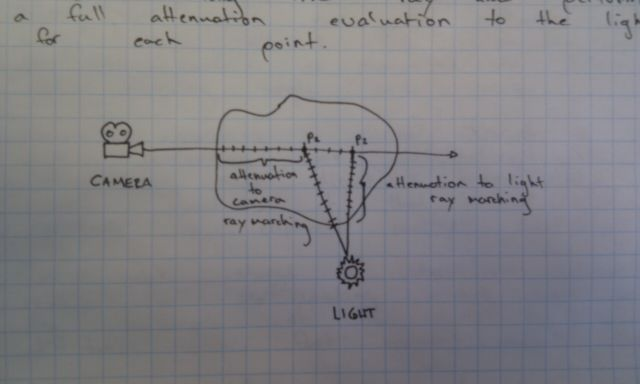
\includegraphics[scale=0.5]{Images/SingleScatteringRayTracing}
	\caption{Solving Single Scattering with Ray Tracing}
\end{figure}

\subsubsection{Photon Mapping Methods}

Photon mapping is a rendering technique which can be used to efficiently compute global illumination in scenes which consist of both solid surfaces and participating media. The photon mapping algorithm calculates global illumination by emitting photons into the scene from the light sources and tracing their paths through the scene as the photons interact with the various surfaces and participating media. When a photon collides with a solid surface, the bidirectional reflectance distribution function of the surface is evaluated to determine the outgoing angle and energy of the photon as it continues through the scene. In order to calculate the interaction of a photon with the participating media, the photon is ray-marched through any participating media volumes. At each step, the phase function of the participating media is evaluated to determine if the photon will scatter and change directions and the absorption cross section is used to calculate the likelihood with which the photon will be absorbed (terminating its traversal of the scene).
\newline \newline
Photons are stored in a photon map at those points where they interact with the surfaces in the scene. Photons are also stored in a photon map when they interact with participating media. For performance reasons, those photons which represent radiance from diffuse, caustic (those photons which have interacted with reflective/refractive surfaces) and participating media sources are normally stored in their own separate maps. These photon maps are typically implemented using kd-trees, such that efficient nearest neighbor queries can be performed (these queries are used for evaluating the amount of radiance at some point within the scene at render time). 
\newline \newline
At each point where a photon interacts with the participating media, it will be either absorbed or scattered. The probability of scattering is denoted by the scattering albedo, $\Lambda$:

\begin{equation}
\Lambda = \frac{\sigma_{s}}{\sigma_{t}}
\end{equation}

Where $\sigma_{s}$ is the scattering coefficient and $\sigma_{t}$ is the transmission coefficient. This scattering albedo can be used to scale the power of a photon after it has scattered. However, this will in many cases result in a large number of low power photons which is computationally inefficient. Instead, Russian roulette\cite{Arvo:1990:PTI:97880.97886} can be used to determine if a photon is scattered or absorbed. This can be accomplished by comparing $\Lambda$ to a random number $\epsilon \in [0,1]$:
\newline \newline
\[
  \text{Given $\epsilon \in [0,1]$} = \left\{ 
  \begin{array}{l l}
    \epsilon \leq \Lambda  & \quad \text{Photon is scattered}\\
    \epsilon > \Lambda & \quad \text{Photon is absorbed}\\
  \end{array} \right.
\]
\newline \newline
In order to evaluate the radiance at some point, on a surface or in a participating media volume, the photon maps are queried. We can estimate the reflected radiance at a surface point using the following:

\begin{equation}
L_{r}(x, w) = \frac{1}{\pi r^{2}}\displaystyle\sum_{p=1}^{N}f_{r}(x,w_{p},w)\Delta\Phi_{p}(x,w_{p})
\end{equation}

To estimate the radiance at some point in a volume a slight modification is required to account for sampling photons within a sphere instead of a disc on a surface:

\begin{equation}
(w\cdot \bigtriangledown)L_{o}(x, w) = \displaystyle\sum_{p=1}^{n}p(x,w_{p},w)\frac{\Delta\Phi_{p}(x,w_{p})}{\frac{4}{3}\pi r^{2}}
\end{equation}

Used in conjunction with ray tracing (to solve for single scattering) photon mapping is an effective technique for computing multiple scattering effects.

\begin{figure}[h!]
	\centering
	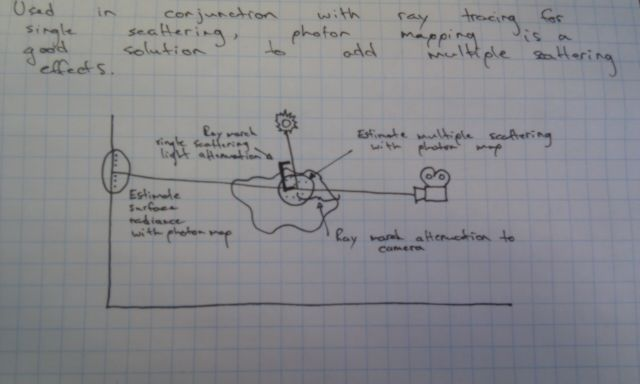
\includegraphics[scale=0.5]{Images/MultipleScatteringWithPhotonMapping}
	\caption{Solving Multiple Scattering using Photon Mapping}
\end{figure}

\section{Related Work}

\subsection{Deep Shadow Maps}

Deep shadow maps \cite{Lokovic:2000:DSM:344779.344958} are a technique which produces high quality shadows for volumetric media such as hair and smoke. In contrast to traditional shadow maps, which store a single depth per pixel, deep shadow maps stores a representation of the transmittance through a pixel at a range of depths. 

Deep shadow maps have the following advantages over traditional shadow maps:

\begin{itemize}

\item Support for transparent surfaces and volumetric primitives such as smoke
\item For the same quality shadows, a smaller shadow map can be used
\item Support for mip-mapping

\end{itemize}

A deep shadow map is a rectangular array of pixels in which every pixel stores a visibility function. Consider a ray that starts at the shadow camera origin and passes through the point (x,y) on the image plane. Some fraction of the light emitted along this ray will be attenuated by surfaces or by volumetric scattering and absorption. The fraction of the light that penetrates to a given depth z is known as the transmittance $\tau$(x,y,z). We refer to $\tau$ as a transmittance function when we wish to consider the transmittance at a fixed image point (x,y) as a function of z. This transmittance is stored in the form of a linked-list of depth/transmittance pairs per pixel. 

\subsection{Opacity Shadow Maps}

The deep shadow map algorithm stores a per-pixel piecewise linear approximation of the transmittance function instead of a single depth which results in a more precise shadow computation than traditional depth based shadow maps. However, this compactness and quality is achieved at the expense of significant up-front processing. In the case of animation, where lights or scene geometry updating, these maps can become costly to compute.

Opacity shadow maps \cite{Kim01opacityshadow} seek to calculate the transmittance function for any point in space using an algorithm which can be hardware accelerated. The opacity shadow map algorithm uses a set of parallel opacity maps which are oriented perpendicular to the light's direction. By approximating the transmittance function with discrete planar maps, opacity maps can be efficiently generated using graphics processing unit hardware. On each opacity map, the scene is rendered from the light's perspective, clipped by the map's depth. Instead of storing depth values, each pixel stores $\Omega$, the line integral of densities along the path from the light to the pixel. The opacity values from adjacent maps are sampled and interpolated, to find the amount of light reaching some point in space, during rendering.

\begin{figure}[h!]
	\centering
	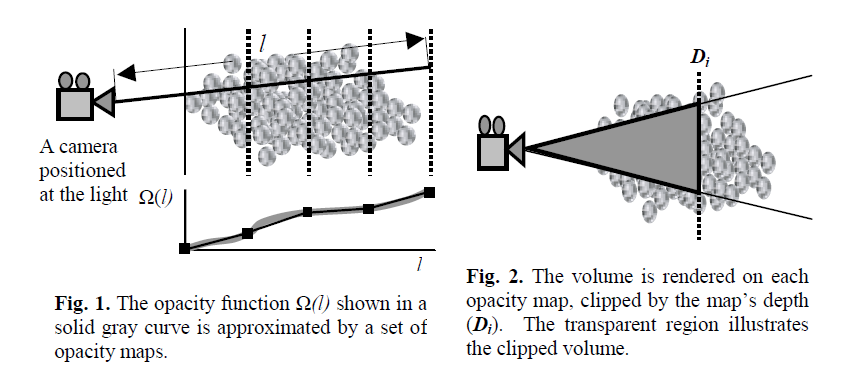
\includegraphics[scale=0.5]{Images/OpacityShadowMaps}
	\caption{Opacity Shadow Maps}
\end{figure}

\subsection{Deep Opacity Maps}

Deep opacity maps \cite{deepopacitymaps08} extend the opacity shadow map concept to improve visual quality while decreasing the number of mapping layers required. This is accomplished by using both traditional shadow mapping and opacity shadow maps in order to create a better distribution of opacity layers. Instead of using slices at regular intervals, depth information (from the traditional shadow map) is used to create opacity layers that vary in depth from the light source on a per-pixel basis. Since the opacity layers are warped to match the scene geometry, significantly fewer layers are needed to achieve sufficient rendering quality.

\begin{figure}[h!]
	\centering
	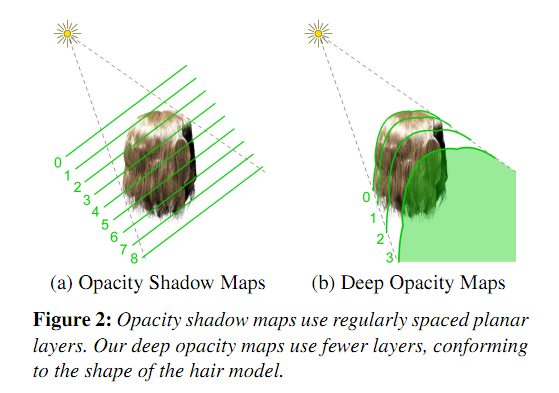
\includegraphics[scale=0.5]{Images/DeepOpacityMaps}
	\caption{Deep Opacity Maps}
\end{figure}

\subsection{Fourier Opacity Mapping}

While the deep shadow maps algorithm is a suitable off line method for calculating lighting in participating media, it can consume an unbounded amount of memory and is, in the basic form, unsuited to be implemented on graphics hardware. Fourier opacity mapping \cite{Jansen:2010:FOM:1730804.1730831} is similar to opacity shadow maps and deep opacity maps in that it can be readily implemented on graphics hardware. However, instead of using discrete sampling planes (uniform or otherwise warped to scene geometry) Fourier opacity mapping stores transmittance information as a set of Fourier co-efficients which can be used to produce a smooth, continuous transmittance value along any light ray. 

\section{The Particle Based Participating Media Rendering Problem}

Our goal is to create an algorithm which can render volumetric lighting effects in a time efficient, physically plausible manner. To be clear, we say those volumetric lighting effects are:

\begin{itemize}

\item Light attenuates as a result of interaction with inhomogeneous participating media
\item Solid objects block light forming volumetric shadows
\item Support for an arbitrary number of lights
\item Support for all conventional computer graphics light types (points, spot, directional)

\end{itemize}

Our rendering technique models inhomogeneous participating media using particle data sets. Particles are used such that our simulation is spatially unbounded and not limited by system memory (as otherwise would be the case for grid based systems).
\newline \newline
These requirements present a unique rendering challenge. We must solve two density integrations for each particle:

\begin{enumerate}
  \item Find the attenuation of the light reaching the camera from a given particle
  \item Find the attenuation of the light reaching a particle from a given light source
\end{enumerate}

We make the observation that use of GPU hardware is an excellent solution to Problem 1. Using alpha blending we can solve this density integration per particle for millions of particles at interactive rates. Even with depth sorting (required to obtain correct blending) this is a relative non issue.
\newline \newline
Furthermore, we have a pre-existing solution\cite{fury2010} to solve motion blur and depth of field. This involves using the geometry shader stage of the GPU pipeline to create point sprites. By varying the characteristics of these sprites we obtain these effects, as detailed in the following pertinent sections.

The rendering process begins with the lighting computation. The lighting data is computed using the CPU for ease of implementation reasons. The data is added to the vertex buffers which represent the particles and then sent to the GPU for the final rendering.

We begin by explaining the lighting process and then outline the process used to create the final image using the GPU.

\subsection{Volumetric Lighting Calculation}

In order to determine how much light reaches a particle from light source we must integrate the density along the light ray between that particle and light source. This presents a challenge for our rendering system, in that because we are modeling the participating media there is no grid which we can perform a ray marching density integration upon. Instead, we use a special formed octree as out density integrator.

\subsubsection{Density Octree}

In order to satisfy the requirement of a spatial data structure which can represent the density of our particle data sets we elect to use an octree.

The density octree is formed by inserting the constituent particles of our data set, subdividing octree cells when a user selected density is achieved. The octree has the useful property of only allocating memory in those areas where there is greater detail in the original particle data set.

The density octree is only built once per frame in which particles or other scene objects change their position, the same density octree is used in turn for each light. In this way, the small setup time associated with creating the density octree is amortized across the number of lighting passes required. 

\begin{figure}[h!]
	\centering
	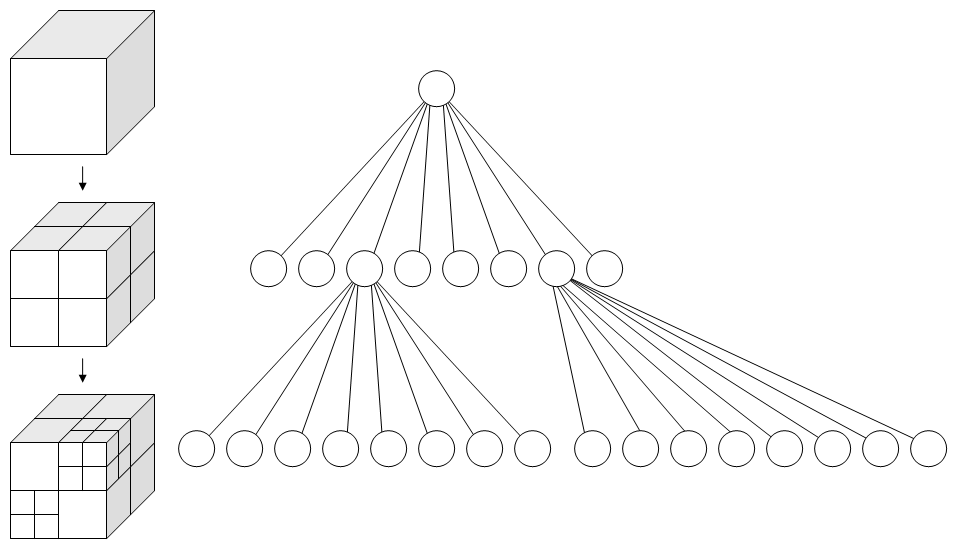
\includegraphics[scale=0.3]{Images/Octree}
	\caption{Octree formed through three subdivisions}
\end{figure}

Each octree node stores the number of particle which reside within the nodes spatial extent.

\subsubsection{Density Octree Smoothing}

<SAY SOMETHING

\subsubsection{Lighting Evaluation}

Integration of the density octree is performed via ray casting. A ray is constructed between some particle and the light source that is currently being evaluated. This ray is then intersected with the nodes of the octree in a top-down manner. This ray casting approach is advantageous in that ray-AABB tests are only required only for those areas of density defined by the density octree. This is in contrast to ray marching, where it is often the case that multiple steps might be performed within a given uniform grid cell. By performing these density evaluations only as necessary, computer memory is accessed less often resulting in better performance. 

Although it would seem necessary to perform intersection testing between the light-particle ray and each particle, we experimentally determined that this is not the case. In fact, performing such exact testing actually results in over-defining the transmittance signal resulting in visually objectionable high frequency noise.

Furthermore, we have found that allowing the user to blend between a uniform density across the entire tree and the per cell density allows a great deal of flexibility in terms of tuning the appearance in terms of details vs. smoothness.

<INSERT OVER DEFINED EXAMPLE GRAPH>

We determine the attenuation by ray casting, counting the number of ray-particle interactions and calculating the attenuation accordingly.

\begin{equation}
particle\:illumination = e^{-ray\:casting\:density\:*\:density\:scaling\:factor}
\end{equation}

\begin{figure}[h!]
	\centering

\begin{algorithmic}
\FORALL{particles} 
	\STATE construct a ray from the particle to the light
	\FORALL{particles (or a subset)} 
		\STATE check ray - particle intersection
		\IF {intersection} 
        			\STATE attenuate light energy
		\ENDIF
		\IF {$light\;energy \leq 0$} 	
        			\STATE break ray-particle intersection checking loop
		\ENDIF
	\ENDFOR
\ENDFOR
\end{algorithmic}

	\caption{Pseudo-code for naive ray-particle testing procedure.}
\end{figure}

\subsection{Ray-Particle Intersection Testing}

Fundamentally speaking, the particle which constitute a point based data set have no size. However, in order to translate them into volumes which can be rendered to pixel on a display, some size must be assigned. While larger sizes reduce the number of particles required to achieved coverage on-screen, they also limit the amount of detail and so some balance regarding particle size must be obtained. We create a logical mapping between the size of the particle used for rasterization and that used for ray-particle intersection tests. We have found that a one to one mapping of particle size in relative units between rasterization size and intersection size is generally optimal. However, this relationship is easily modified and can be configured by end users.

We make the fundamental observation that, although it may be possible to create an alternative method which uses data buckets or a formula driven approach (such a Fourier analysis) to create an interpolation strategy, it is necessary to compute a complete and accurate lighting evaluation for each particle being rendered.

\subsubsection{Intersection Algorithm (Ray-Sphere)}

We use the following optimized ray-sphere intersection\cite{RTR3}:

\subsubsection{Intersection Algorithm (Ray-AABB)}

We use the following optimized ray-AABB intersection:

<INSERT CITATION FOR SHIRLEY INTERSECTION ALGORITHM>

\subsection{Solid Geometry Volumetric Shadowing}

So far our discussion has pertained primarily to the calculating the interaction of light with participating media. However, we also want to take into account the presence of solid surfaces within the scene. In order to achieve this aim, we build a Bounding Volume Hierarchy BVH) on the solid geometry. Prior to conducting a full attenuation calculation using the density octree, the given particle-light ray in question is tested against the solid geometry BVH. If the ray intersects some solid surfaces then no light will be reaching that point and it can be concluded that the illumination for that particle is zero without further computational expense.  

<INSERT DIAGRAM SHOWING AN EXAMPLE OF THIS>

\subsection{Forward Density Integration using GPU Hardware}

In order to determine the amount of light reaching the camera from some particle we must evaluate the out going radiance from each point taking into account the attenuation due to those particles which occlude the particle which we are evaluating. In order to render correctly alpha blended particles using the GPU we must sort the vertices that represent those particles. Sorting is performed based upon the vertices distance to the camera. Once the particles are sorted they are uploaded to the GPU in order to be rendered. 

A custom geometry shader is used which expands each single vertex into a set of four vertices which represent a quad facing the camera centered around the original vertex position. By varying the size of the generated quad it is possible to have user selectable particle sizes. Furthermore, because UV coordinates for the quad are generated by geometry shader it is possible to map arbitrary particle color and opacity maps to the quad. Having adjustable particles sizes is convenient in that it allows for smoothing to be performed by using larger than a single pixel, low opacity particles.

We further detail the methods by which we produce two characteristic cinematic effects, motion blur and depth of field, which are essential for compositing particle renderings into special effects shots for film and television.

\begin{figure}[h!]
	\centering
	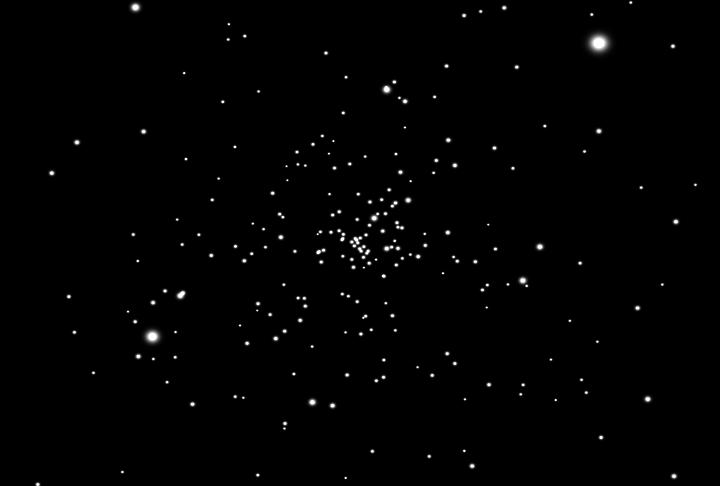
\includegraphics[scale=0.5]{Images/FuryBasic}
	\caption{Example of a simple GPU particle rendering}
\end{figure}

\begin{figure}[h!]
	\centering
	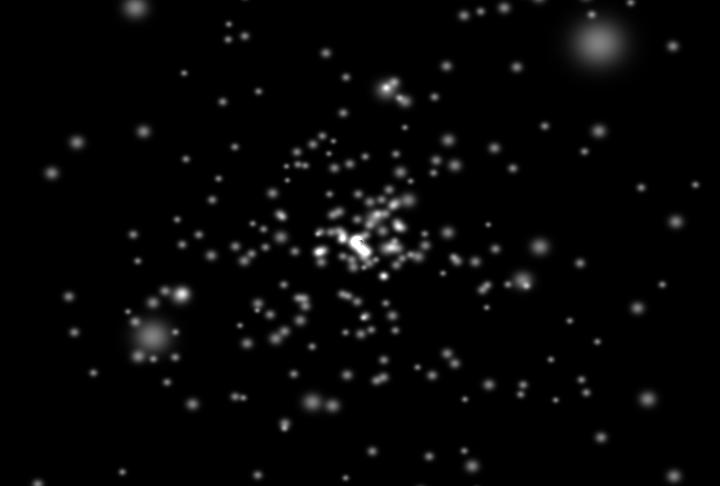
\includegraphics[scale=0.5]{Images/FuryLargePoints}
	\caption{Example of rendering larger particles using the geometry shader scaling procedure}
\end{figure}

\subsubsection{Motion Blur}

Motion blur is the blur in an image which results from the rapid movement of the camera or the scene being viewed such that during a single exposure multiple views of the scene occur. Using the geometry shader stage it is possible to efficiently create such a motion blur effect. This is accomplished by modifying the shape of the quads that are produced. By creating rectangular quads of varying dimensions, where elongation relates to greater particle speed, a motion blur effect is achieved.

\begin{figure}[h!]
	\centering
	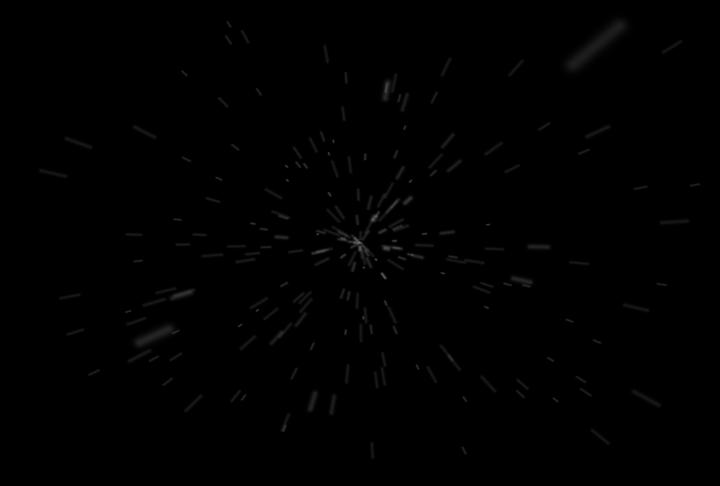
\includegraphics[scale=0.5]{Images/FuryMotionBlur}
	\caption{Example of the motion blur effect created using the geometry shader}
\end{figure}

\subsubsection{Depth of Field}

Depth of field is the distance between the nearest and furthest objects in a scene that appear acceptably in focus in a rendered image. By adjusting the depth of field it is possible to direct the viewers attention to that potion of the scene which is in focus. In a manner similar to that which is used for rendering motion blur, it is possible to use the geometry shader to create a depth of field effect. This is accomplished by varying the size of the quad based upon its distance from the focal point. Additionally, the dropoff curve which controls the particle opacity is modified to simulate the effects of depth of field.

\begin{figure}[h!]
	\centering
	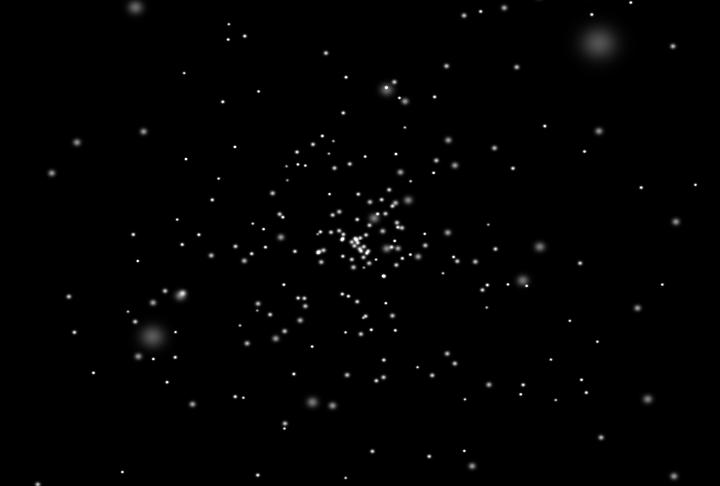
\includegraphics[scale=0.5]{Images/FuryDepthOfField}
	\caption{Example of the motion blur effect created using the geometry shader. Note how particles in the foreground appear out of focus.}
\end{figure}

\subsection{Algorithmic Efficiency}

In the naive formulation, our algorithm would be expected to run in $O(n^{2})$ time. However, we can improve this expected run time in several ways:

\begin{enumerate}

  \item Early termination: If the attenuation (as calculated by ray-particle intersection tests) has reduced transmission to zero, then there is no reason to continue computation. In such a scenario, the remaining ray-particle intersections can be aborted in order to save computations.

For participating media that is characterized by a significant density, this alone improvement alone can significantly improve run times, as light will be attenuated to zero well before the total number of computations is performed.

  \item Spatial Tree Structures: Ray casting can be optimized with any tree structure that would commonly be used for traditional ray tracing such as an octree or kd-tree.

It is yet to be seen if the time required to build a tree on the particle data set (which will be changing per frame) out weighs the time saved by using such a structure.

\item Level of Detail: In regions further from the camera, it is not necessary that the lighting calculations be as accurate, as viewers will not be able to see detail in those areas. Using our algorithm it is easy to adjust the level of detail used by making the percentage of total particles used in ray-particle checks a function of the distance to the camera. In this way, full details are only computed as necessary.

\item Parallelism: Because each particle calculation is independent, our algorithm exhibits a high degree of parallelism which can be exploited on multi-core or GPU hardware.

\end{enumerate}

With these optimizations, notably the use of a tree based data structure, it is possible to reduce the expected run-time to $O(n\;log\;n)$.

Thus we have an algorithm which calculates lighting on a per particle basis with negligible memory overhead and has several computational optimizations.

\subsection{Spatial Partitioning Tree}

\subsection{Multi-threading Support}

In order to take full advantage of modern multi-core processors, we implement our solution using the Intel Threading Building Blocks (TBB) code library. This library exposes a number of convenient programming constructs that facilitate allowing code to scale workloads across multiple cores and processors. The primary section of our code that benefits from this optimization is the ray traversal of the density octree. Since the density octree is not modified in the course of rendering a single frame, meaning that only read operations are performed on the memory which represents the tree, it is relatively trivial to parallelize this process. We apply the TBB parallel for construct which automatically handles the assignment of threads to each available core or processor in order to optimize throughput. In this way we are able to better utilize the available computing resources to the extent that the available bandwidth will allow.

\section{Performance Evaluation}

We evaluate the performance of the above described system against the following metrics. Our point of comparison is Krakatoa, an industry standard particle rendering system produced by Thinkbox Software, which has been used in the production of numerous commercial films and commercials.

\subsection{Image Quality vs. Particle Count}

Note how Krakatoa requires significantly more particles to achieve as smooth a lighting solution. As a result of requiring more particles, Krakatoa takes more time to produce the same output quality. 

\subsection{Time vs. Particle Count}

Using our lighting algorithm, time increases linearly with the number of particles in the scene.

\subsection{Time vs. Number of Lights}

Using our system, the time increase associated with adding more lights is linear.

\subsection{Time vs. Image Size}

Our lighting, motion blur and depth of field calculations are independent of ouput image size. As such, no more computation time is required for higher resolution output.

\subsection{Example Images}

\section{Conclusion}

\subsection{Conclusions}



\subsection{Summary of Contributions}

\subsection{Future Research}

We have identified the following areas as potential avenues for future research.

\subsubsection{Cache Efficient Octree}

At the core of our system is the octree data structure which is used to create the density evaluator. As such, any improvements that can be made to the efficiency of the octree will directly also improve our algorithm run times. One such improvement can come in the form of a cache efficient octree. On modern central processing units, where memory latency is hidden using special on processor caches, significant speed improvements can be obtained by specifically designing data structures which take advantage of such caches. We would be interested to revisit our implementation and determine whether additional performance could be achieved by using such specially designed octree implementations.

\subsubsection{GPU Implementation of Octree}

\subsubsection{Automatic Level of Detail}



\pagebreak[4]
\bibliography{Thesis}{}
\bibliographystyle{plain}

\end{document}